\documentclass{article}
\usepackage[utf8]{inputenc}
\usepackage{amsmath}
\usepackage{enumitem}
\usepackage[a4paper, total={7in, 10in}]{geometry}
\newlist{subquestion}{enumerate}{1}
\setlist[subquestion,1]{label=(\alph*)}
\usepackage{lipsum}
\usepackage{fancyhdr}
\pagestyle{fancy}
\usepackage{tikz,tkz-tab}
\documentclass{article}
\usepackage{fourier}
\title{DM Mathématiques}
\author{BONNET Mattéo et LURIN Paul }
\date{Samedi 9 janvier} 

\begin{document} \\
    \begin{exo2}
        \maketitle 
        \underline{\textbf{\large{Exercice 1}}} \\ \\
        
            Soit $n$ un entier naturel non nul. \\
            On cherche à déterminer le nombre de solutions de l'équation $x^{n}(1-x)=1$ \\ \\
            On considère la fonction $f(x) = x^{n}(1-x)-1$ tel que $x\in{\rm I\!R}$, et $n\in{\rm I\!N^*}$.\\
            La fonction est dérivable sur ${\rm I\!R}$. \\
            On cherche à déterminer la dérivée $f'(x)$. \\
            
                $f'(x)=nx^{n-1}(1-x)-xn$ \\
                
                $f'(x)=x^{n-1}[n(1-x)-x]$ \\
                
                $f'(x)=x^{n-1}[n-x(n+1)]$ \\ \\
            On remarque que : \\
            
            - $x^{n-1}>0$ si $x>0$ \\
            
            - $x^{n-1}<0$ si $x<0$ \textbf{et} si $n$ est pair. \\ \\
            On procède par disjonction des cas. \\
            On séparera le cas : \\ 
            - où $n$ est pair, \\
            - où $n$ est impair. \\ \\
            
            \textbf{\large{1. n est pair}} \\ \\
            
                Ici, on cherchera le nombre de solutions de l'équation $x^{n}(1-x)=1$, pour tout $n\in{\rm I\!N^*}$ et pair. \\
                On décide de calculer les limite de $f(x)$, afin d'étudier les variations de la fonction $f(x)$, lorsque $n$ est pair.\\
                Lorsque $n$ est pair : \\
                
                - si $x>0$, $x^{n-1}>0$ \\
                
                - si $x<0$, $x^{n-1}<0$ \\
                
                - si $x=0$, $x^{n-1}=0$ \\ \\
                On cherche une valeur de $x$ tel que $n-(n+1)x=0$ : \\
                
                $n-(n+1)x=0$ \\
                
                $\Leftrightarrow$ $n=(n+1)x$ \\
                
                $\Leftrightarrow$ $x=\frac{n}{n+1}$ \\ \\
                Donc, lorsque $x=\frac{n}{n+1}$, $n-(n+1)x=0$. \\ \\ 
                Aussi, si $x<\frac{n}{n+1}$, $n-(n+1)x>0 $ \\ \\
                Inversement, si $x>\frac{n}{n+1}$, $n-(n+1)x<0 $ \\ \\
                On dresse le tableau de variations suivant : \\
                
                
          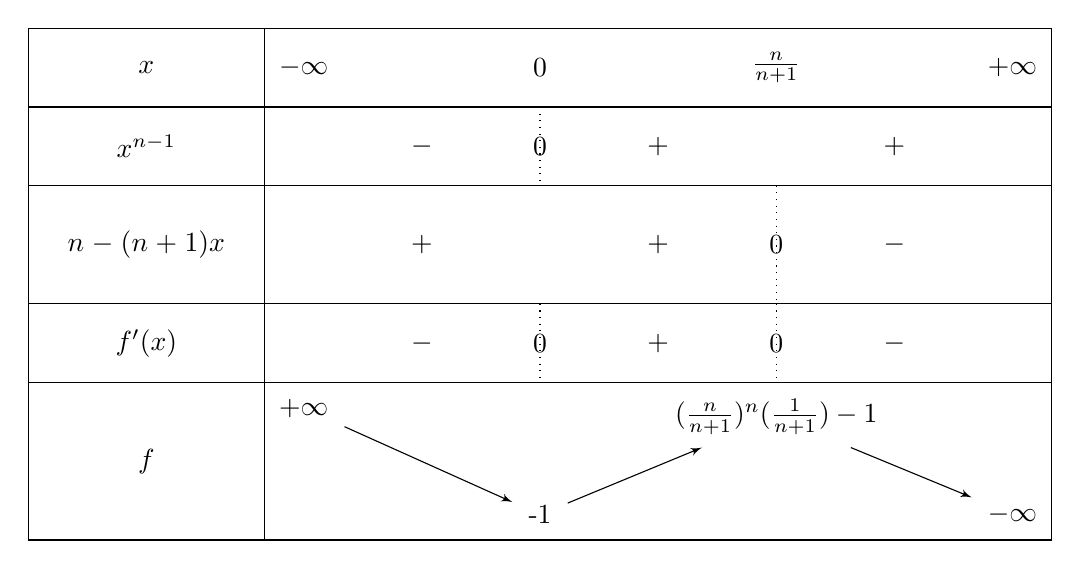
\begin{tikzpicture}
            \tkzTabInit[lgt = 3]{$x$/1 , $x^{n-1}$/1, $n-(n+1)x$/1.5, $f'(x)$/1, $f$/2}{$-\infty$, $0$, $\frac{n}{n+1}$, $+\infty$}
                \tkzTabLine{, -, z, +, , +}
                \tkzTabLine{, +, , + , z, -}
                \tkzTabLine{, -, z, + , z, -}
                \tkzTabVar{+/$+\infty$, -/-1, +/$(\frac{n}{n+1})^{n}(\frac{1}{n+1})-1$, -/$-\infty$}
        \end{tikzpicture} \\ \\           
        Calcul de $f(0)$ : \\
        
        $f(0) = 0^{n}(1-0)-1$ \\ \\
        Donc $f(0) = -1$ \\ \\
        Calcul de $f(\frac{n}{n+1})$ : \\
        
        $f(\frac{n}{n+1}) = (\frac{n}{n+1})^{n}(1-\frac{n}{n+1})-1$ \\ \\
        Donc $f(\frac{n}{n+1}) = (\frac{n}{n+1})^{n}(\frac{1}{n+1})-1$ \\ \\  \\    
        Ensuite, on calcule les limites de la fonction $f(x)$ en $+\infty$ et $-\infty$, tout en sachant que $n$ est pair :


    \[\
     \left.
        \begin{array}{ll}
            \lim\limits_{x \rightarrow -\infty} x^{n} = +\infty \\
            \lim\limits_{x \rightarrow -\infty} 1-x = +\infty
        \end{array}
    \right \} \left.
        \begin{array}{ll}
        \lim\limits_{x \rightarrow -\infty} x^{n}(1-x) = +\infty \\ \\
            \lim\limits_{x \rightarrow -\infty} -1 = -1 
        \end{array}
    \right \}\lim\limits_{x \rightarrow -\infty} x^{n}(1-x) -1 = +\infty
    \]
    
    \\ \\
    
    \[\
     \left.
        \begin{array}{ll}
            \lim\limits_{x \rightarrow +\infty} x^{n} = +\infty \\
            \lim\limits_{x \rightarrow +\infty} 1-x = -\infty
        \end{array}
    \right \} \left.
        \begin{array}{ll}
        \lim\limits_{x \rightarrow +\infty} x^{n}(1-x) = -\infty \\ \\
            \lim\limits_{x \rightarrow +\infty} -1 = -1
        \end{array}
    \right \}\lim\limits_{x \rightarrow +\infty} x^{n}(1-x) -1 = -\infty
    \] \\ \\ 
        On souhaite alors déterminer le signe de $(\frac{n}{n+1})^{n}(\frac{1}{n+1})-1$ \\ \\
        Puisque $\frac{n}{n+1}<1$, alors $(\frac{n}{n+1})^{n}<1$. \\ \\
        Puisque $\frac{1}{n+1}<1$, alors $(\frac{n}{n+1})^{n}(\frac{1}{n+1})<1$.\\ \\ 
        On en déduit donc que $(\frac{n}{n+1})^{n}(\frac{1}{n+1})-1 < 0$\\ \\ \\
        La fonction f(x) est dérivable donc continue, strictement décroissante sur l'intervalle $]-\infty;0]$, et à valeurs dans $[-1;+\infty[$. \\
        Or, $0\in[-1;+\infty[$ donc, d'après le corollaire du théorème des valeurs intermédiaires, $f(x) = 0$ admet une unique solution sur l'intervalle $]-\infty;0]$. \\
        La fonction f(x) est dérivable donc continue sur l'intervalle $[0;+\infty[$, et à valeurs dans $]-\infty;-1]$ et son maximum est atteint en  $(\frac{n}{n+1})^{n}(\frac{1}{n+1})-1$. \\Or, on a démontré que la valeur de ce maximum était négative. \\ Donc, sur l'intervalle $[0;+\infty[$, la fonction $f(x)$ est strictement inférieure à $0$.\\
        Donc, quand n est pair, on en déduit que la fonction f(x) admet une unique solution, tel que f(x) = 0. \\
        
                     \textbf{\large{2. n est impair}} \\ \\
                     
                Ici, on cherchera le nombre de solutions de l'équation $x^{n}(1-x)=1$, pour tout $n\in{\rm I\!N^*}$ et impair. \\
                On décide de dresser un tableau de variations, afin d'étudier les variations de la fonction $f(x)$, lorsque $n$ est impair.\\
                Lorsque $n$ est impair, $x^{n-1}>0$. Le signe de la dérivée est donc celui de $n-(n+1)x$. \\ \\
                On sait que lorsque $x=\frac{n}{n+1}$, alors $n-(n+1)x=0$.\\ \\
                Aussi, si $x<\frac{n}{n+1}$, $n-(n+1)x>0 $ \\ \\
                Inversement, si $x>\frac{n}{n+1}$, $n-(n+1)x<0 $ \\ \\
                On dresse le tableau de variations suivant : \\
                
                
          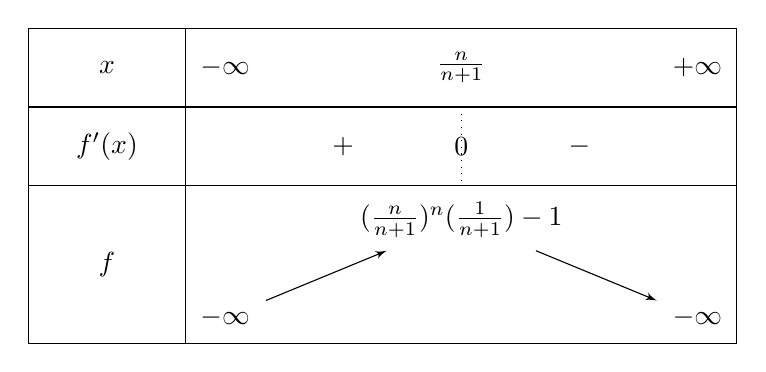
\begin{tikzpicture}
            \tkzTabInit{$x$/1 , $f'(x)$/1, $f$/2}{$-\infty$, $\frac{n}{n+1}$, $+\infty$}
                \tkzTabLine{, +, z, -}
                \tkzTabVar{-/$-\infty$, +/$(\frac{n}{n+1})^{n}(\frac{1}{n+1})-1$, -/$-\infty$}
        \end{tikzpicture} \\ \\           
        Calcul de $f(\frac{n}{n+1})$ : \\
        
        $f(\frac{n}{n+1}) = (\frac{n}{n+1})^{n}(1-\frac{n}{n+1})-1$ \\ \\
        Donc $f(\frac{n}{n+1}) = (\frac{n}{n+1})^{n}(\frac{1}{n+1})-1$ \\ \\  \\    
        Ensuite, on calcule les limites de la fonction $f(x)$ en $+\infty$ et $-\infty$, tout en sachant que $n$ est impair :
    \[\
     \left.
        \begin{array}{ll}
            \lim\limits_{x \rightarrow -\infty} x^{n} = -\infty \\
            \lim\limits_{x \rightarrow -\infty} 1-x = +\infty
        \end{array}
    \right \} \left.
        \begin{array}{ll}
        \lim\limits_{x \rightarrow -\infty} x^{n}(1-x) = -\infty \\ \\
            \lim\limits_{x \rightarrow -\infty} -1 = -1 
        \end{array}
    \right \}\lim\limits_{x \rightarrow -\infty} x^{n}(1-x) -1 = -\infty
    \]
    
    \\ \\
    
    \[\
     \left.
        \begin{array}{ll}
            \lim\limits_{x \rightarrow +\infty} x^{n} = +\infty \\
            \lim\limits_{x \rightarrow +\infty} 1-x = -\infty
        \end{array}
    \right \} \left.
        \begin{array}{ll}
        \lim\limits_{x \rightarrow +\infty} x^{n}(1-x) = -\infty \\ \\
            \lim\limits_{x \rightarrow +\infty} -1 = -1
        \end{array}
    \right \}\lim\limits_{x \rightarrow +\infty} x^{n}(1-x) -1 = -\infty
    \] \\ \\ 
        On souhaite alors déterminer le signe de $(\frac{n}{n+1})^{n}(\frac{1}{n+1})-1$ \\ \\
        Puisque $\frac{n}{n+1}<1$, alors $(\frac{n}{n+1})^{n}<1$. \\ \\
        Puisque $\frac{1}{n+1}<1$, alors $(\frac{n}{n+1})^{n}(\frac{1}{n+1})<1$.\\ \\ 
        On en déduit donc que $(\frac{n}{n+1})^{n}(\frac{1}{n+1})-1 < 0$ \\ \\ \\
        La fonction f(x) est dérivable donc continue sur l'intervalle $]-\infty;+\infty[$, et à valeurs dans $]-\infty;(\frac{n}{n+1})^{n}(\frac{1}{n+1})-1]$ et son maximum est donc atteint en  $(\frac{n}{n+1})^{n}(\frac{1}{n+1})-1$. \\ Or, on a démontré que ce maximum était négatif. \\ Donc, sur l'intervalle $[0;+\infty[$, la fonction $f(x)$ est strictement inférieure à $0$. \\
        Donc, quand n est impair, on en déduit que la fonction $f(x)$ n'admet aucune solution, tel que $f(x) = 0$. \\ \\ \\
        
         \textbf{\large{CONCLUSION}} \\ \\ 
         
        Le but de cet exercice est de justifier le nombre de solutions de l'équation $x^{n}(1-x)=1$, pour tout $x\in{\rm I\!R}$ et $n\in{\rm I\!N^*}$. \\
        Pour cela, on a défini la fonction $f(x)=x^{n}(1-x)-1$, et on a cherché pour quelles valeurs de $x$ la fonction était égale à 0. Cela revenait donc à chercher le nombre de solutions de l'équation $x^{n}(1-x)=1$. \\ \\
        Grâce à une disjonction des cas, on a pu déterminer les affirmations suivantes : \\ 
        - Lorsque $n$ est pair, l'équation $x^{n}(1-x)=1$ possède une unique solution, tel que $x\in{\rm I\!R}$, et $n\in{\rm I\!N^*}$. \\
        - En revanche, lorsque $n$ est impair, l'équation $x^{n}(1-x)=1$ ne possède aucune solution, tel que $x\in{\rm I\!R}$, et $n\in{\rm I\!N^*}$. \\ 
        On remarque que les résultats obtenus grâce à une calculatrice concordent avec les affirmations démontrées. \\ \\ \\ \\ \\ \\ \\ \\
        
        Travail réalisé par Paul Lurin et Mattéo Bonnet, T°8.
        
         
           
    \end{exo2}



   
    

        
        
        
        
        
\end{document}